\documentclass{amsart}

\input{../preamble_general.tex}

\author{Jalen Chrysos}
\title{Embedded Graphs (with Solutions)}

\begin{document}
	\maketitle 
		We've talked about planar graphs, graphs that can be embedded in $\R^2$ without edges crossing. But what if we replace $\R^2$ by some other surface $S$, for example a torus?\\
	%	We've learned that if a graph $G$ is embedded in the plane, then it satisfies Euler's formula:
	%	$$
	%	V - E + F = 2
	%	$$
	%	where $V$ is the number of vertices of $G$, $E$ is the number of edges, and $F$ is the number of faces. We've also seen that $G$ can be embedded in the plane if and only if $G$ does not contain $K_5$ or $K_{3,3}$ as minors.\\
	%	
	%	\underline{\textbf{Question}}: For a given topological space $S$, what can we say about graphs embedded in $S$?\\
	
	\noindent Technical note: we only consider \textit{cellular embeddings}, which are embeddings of $G$ such that the faces of $G$ are homeomorphic to disks---informally, they have no holes.\\
	%	
	%	$$\textbf{DIAGRAM: CELLULAR VS NONCELLULAR EMBEDDING}$$
	
	\noindent 
	If $G$ has a cellular embedding into $S$, it may not be that $V-E+F=2$, but it is true that $V-E+F$ is some constant depending on $S$ (and not on $G$), which we denote $\chi(S)$:
	$$
	V - E + F = \chi(S).
	$$
	$\chi(S)$ is called the \textbf{\textit{Euler characteristic}} of $S$. In practice it can be computed just by knowing this fact and picking a fairly simple graph with a cellular embedding into $S$.\\
	
	\noindent \textbf{Problem 1}: Compute the Euler characteristics of the following surfaces:
	\begin{enumerate}[(i)]
		\item Plane
		\item Sphere
		\item Torus
		\item $2$-holed torus\\
	\end{enumerate}
	
		\noindent \textbf{Problem 2}: Suppose a simple graph $G$ has a cellular embedding into $S$.
		\begin{enumerate}[(a)]
			\item Show that $E\leq 3(V-\chi(S))$.
			\item Suppose that the shortest cycle in $G$ has length $k$. Show that 
			$$
			E \leq \frac{k}{k-2} (V-\chi(S)).
			$$
		\end{enumerate}
		\vspace{0.1cm}
		
		\textbf{Solution}: Using the fact that $V - E + F = \chi(S)$, the given fact is equivalent to 
		$$
		E \leq \frac{k}{k-2}\cdot (V-\chi(S)) \;\iff \; 	E \leq \frac{k}{k-2}\cdot (E-F) \; \iff \; kF \leq 2E.
		$$
		This holds by double-counting: each edge appears in exactly two faces, and each face contains at least $k$ edges.\\
		
		\noindent \textbf{Problem 3}: What is the highest $n$ such that $K_n$ has a cellular embedding into the torus?\\
		
		\textbf{Solution}: In $K_n$, the shortest cycle has $3$ edges, so in the terms of problem 2 we have $k\geq 3$ for every embedding. And $\chi(T)=0$. Thus $E\leq 3V$ by problem 2. Computing $E,V$ in terms of $n$ yields
		$$
		{n \choose 2} \leq 3 n \; \iff \; n \leq 7
		$$
		so theoretically $7$ is the maximum.\\
		
		In fact, $K_7$ \textit{does} embed into $T$, though in a very non-obvious way. Here is an example of such a cellular embedding:\\
		
		\begin{figure}[h]
			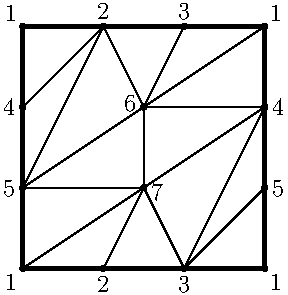
\includegraphics[width=6cm]{./Asymptote_Figs/K7Torus1.pdf}
		\end{figure}
		
		\newpage 
		
		\noindent \textbf{Problem 4}: For which $m,n$ does $K_{m,n}$ have a cellular embedding into the torus?\\
		
			In a bipartite graph, there are no odd cycles. Thus, the shortest possible cycle has length $k=4$, so by problem 2 we have
		$$
		E \leq 2V \; \iff \; mn \leq 2(m+n) \; \iff \; (m-2)(n-2)\leq 4.
		$$
		This restricts the possibilities for $m,n$ to 
		
		\begin{center}
			\begin{tabular}{c|c|c|c|c|c|c|}
				& $2$ & $3$ & $4$ & $5$ & $6$ &$7$ \\
				\hline 
				$2$ & & & & & & \\
				\hline
				$3$ & & & & & & N \\
				\hline
				$4$ & & & & N & N & N\\
				\hline
				$5$ & & & N&N & N&N \\
				\hline
				$6$ & & &N & N&N & N\\
				\hline
				$7$ & & N & N &N &N &N \\
				\hline
			\end{tabular}
		\end{center}
		
		Now it remains to show that all of the blank squares are possible, i.e. that $K_{2,n}$, $K_{3,6}$, and $K_{4,4}$ all admit cellular embedding into the torus. Examples of each of these are shown below:\\
		
		\begin{minipage}{0.3\textwidth}
			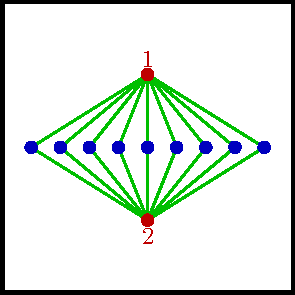
\includegraphics[width=0.9\textwidth]{./Asymptote_Figs/K2nTorus.pdf}
		\end{minipage}
		\begin{minipage}{0.3\textwidth}
			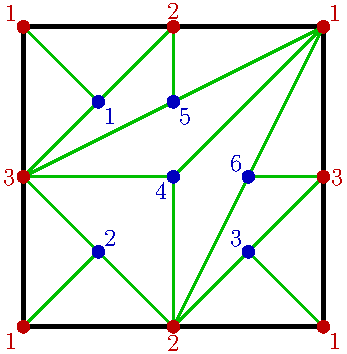
\includegraphics[width=\textwidth]{./Asymptote_Figs/K36Torus.pdf}
		\end{minipage}
		\hspace{0.3cm}
		\begin{minipage}{0.3\textwidth}
			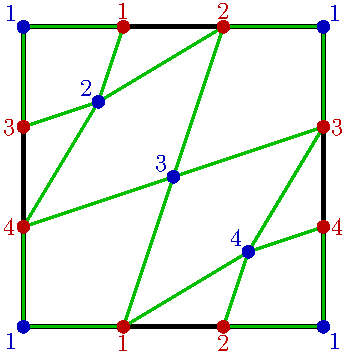
\includegraphics[width=\textwidth]{./Asymptote_Figs/K44Torus.pdf}
		\end{minipage}
		
%		This is beyond our abilities to prove, but Robertson and Seymour proved in 2004 that for any surface $S$, there is some finite set $\G(S)$ of graphs such that $G$ can be cellularly embedded into $S$ if and only if it contains no graph in $\G(S)$ as a minor. For planar graphs, as we saw, $\G(\R^2)=\{K_5,K_{3,3}\}$. For the torus, $\G(T)$ is still not fully known, but it is known that it contains at least 17,000 graphs.\\
		
		
	
\end{document}